We organize context compression failures by the earliest stage at which they arise: {\fone}, {\ftwo}, and {\fthree}, as shown in Figure~\ref{fig:failure_modes_taxonomy}.

% \begin{figure*}[t]
%     \centering
%     \captionbox{A temporal taxonomy of context compression failures. Failures are classified by the earliest point at which they occur in the compression pipeline.\label{fig:failure_modes_taxonomy}}[0.48\textwidth]{%
%     \makebox[\linewidth][l]{%
%         \raisebox{-0.3mm}[0pt][0pt]{%
%             \scalebox{1}[1.1]{%
%                 
\includegraphics[width=\linewidth]{figures/section5.pdf}%
%             }%
%         }%
%     }%
%     \vspace{-.2cm}
% }
%     \hfill
%     \captionbox{Domain-specific context compression regimes, contrasting setup, workflow, interaction loop, dominant risks, and strategy choices.\label{fig:domain_specific_regimes}}[0.49\textwidth]{%
%         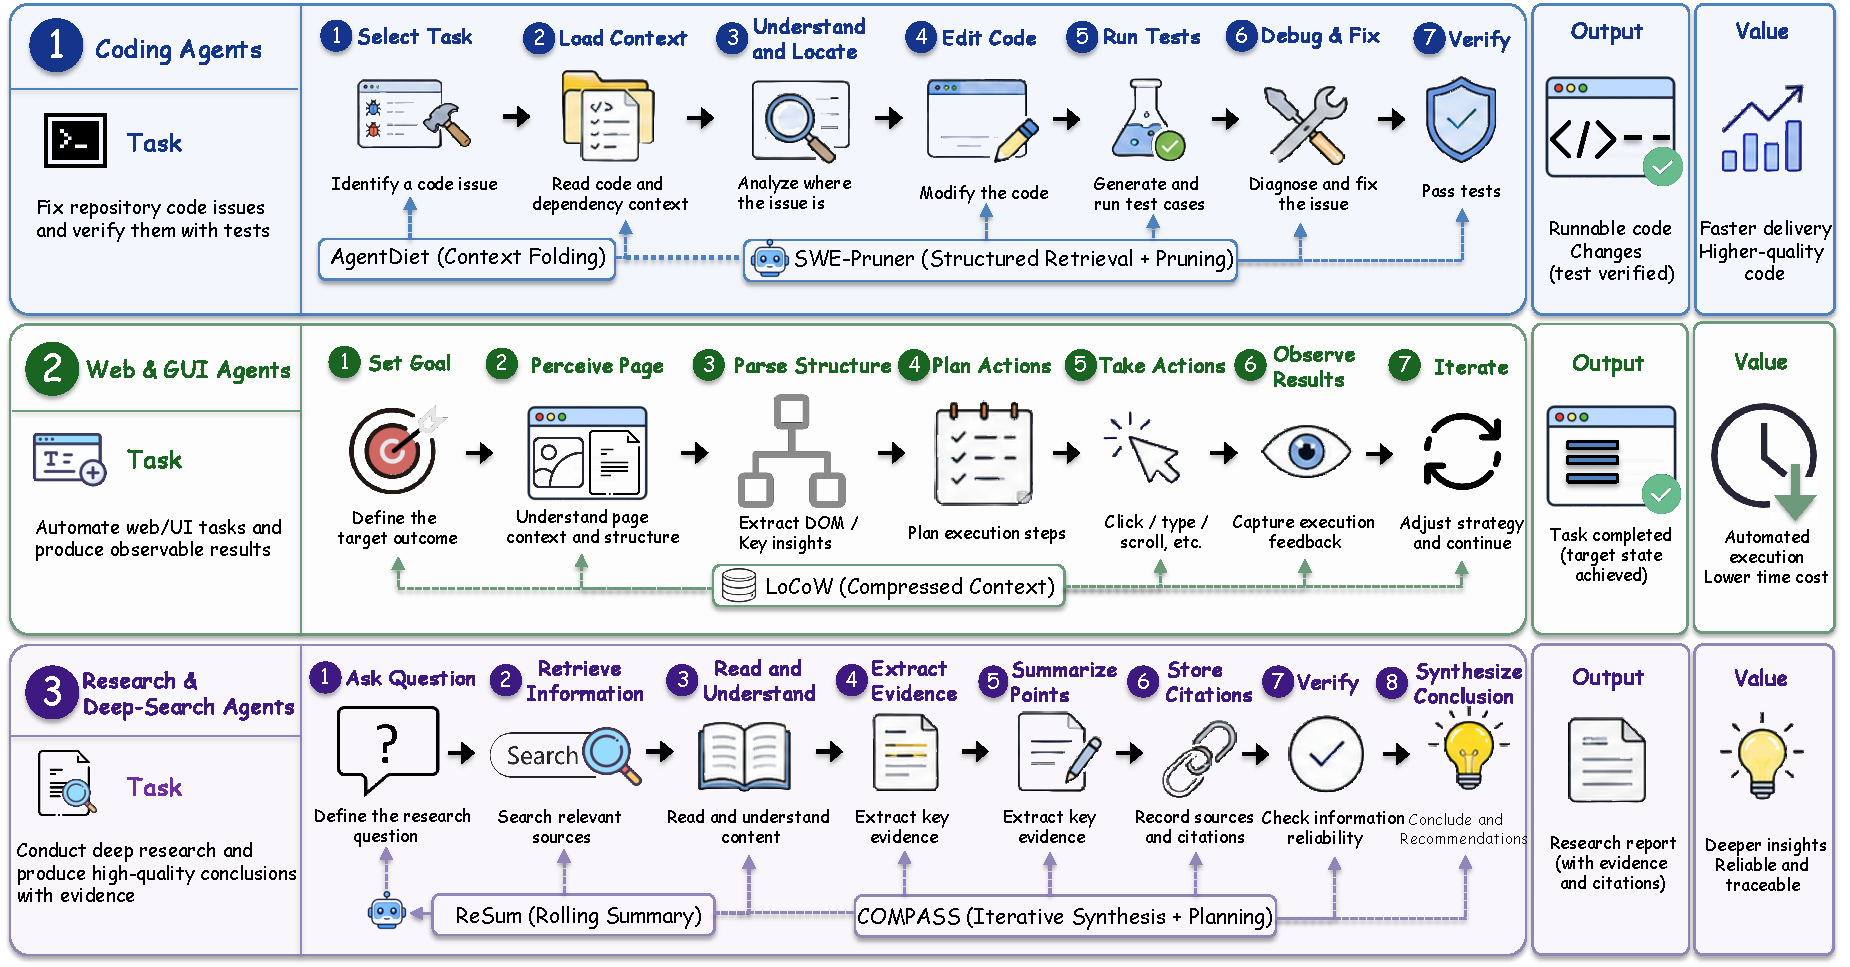
\includegraphics[width=.85\linewidth]{figures/section6.pdf}
%         \vspace{-.2cm}
%     }
% \vspace{-.2cm}
% \end{figure*}





% \begin{figure*}[t]
%     \centering
%     
\includegraphics[width=0.5\textwidth]{figures/section5.pdf}
%     \vspace{-.2cm}
%     \caption{A temporal taxonomy of context compression failures. Failures are classified by the earliest point at which they occur in the compression pipeline: {\fone}, {\ftwo}, and {\fthree}.}
%     \label{fig:failure_modes_taxonomy}
% \end{figure*}

% \begin{figure*}[ht]
%     \centering
%     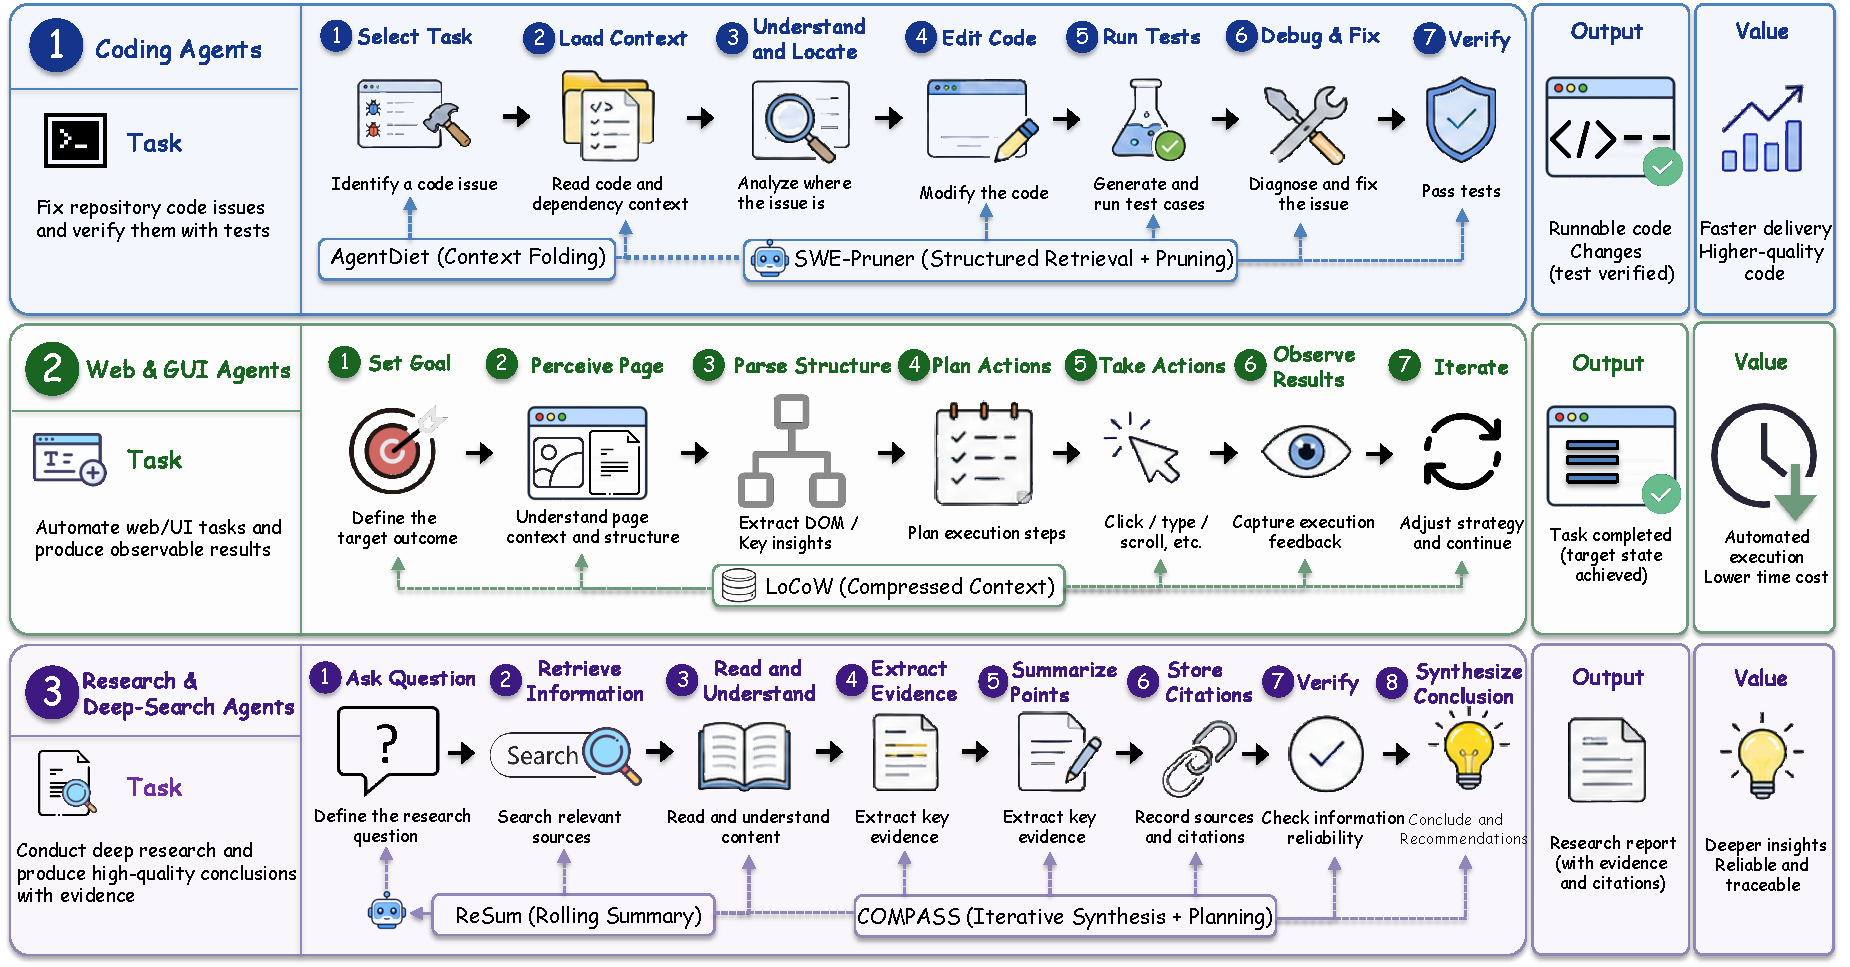
\includegraphics[width=0.5\textwidth]{figures/section6.pdf}
%     \vspace{-.2cm}
%     \caption{Domain-specific context compression regimes for coding, web/GUI, and research agents. The figure contrasts each domain's setup, workflow, interaction loop, dominant risks, and contextualized strategy choices.}
%     \label{fig:domain_specific_regimes}
% \end{figure*}

\begin{table*}[ht]
\centering
\footnotesize
\setlength{\tabcolsep}{4pt}
\setlength{\aboverulesep}{0.2ex}
\setlength{\belowrulesep}{0.2ex}
\renewcommand{\arraystretch}{0.98}
\begin{tabularx}{\textwidth}{@{}>{\raggedright\arraybackslash}p{2.2cm} >{\raggedright\arraybackslash}X >{\raggedright\arraybackslash}X >{\raggedright\arraybackslash}X >{\raggedright\arraybackslash}X@{}}
\toprule
\textbf{System} & \textbf{Select ($S$)} & \textbf{Compress ($\Phi$)} & \textbf{Store ($M$)} & \textbf{Recover ($R$)} \\
\midrule
\textbf{Claude Code} & Reactive, threshold-based selection. & Auto-compaction of prior interaction history. & Compacted state retained in active context. & Implicit recovery via continued execution. \\
\midrule
\textbf{Cursor} & Retrieval-first selection of files, code blocks, and rules. & Relevance filtering and contextual assembly. & Repository index, project rules, and workspace context. & Re-injection of retrieved files, rules, and evidence. \\
\midrule
\textbf{OpenAI Codex} & Task-grounded selection over files, instructions, and threads. & Session continuation and workspace grounding. & Task threads, instruction files, and repository state. & Recovery through continued threads and file re-access. \\
\bottomrule
\end{tabularx}
\vspace{-.2cm}
\caption{Pipeline-level comparison of recent production-grade coding agents, organized by the stages in Section~\ref{subsec:unified_pipeline}.}
\label{tab:coding_agents_pipeline}
\vspace{-.4cm}
\end{table*}

\noindent\textbf{\fone} refers to failures that arise before compression itself, when the system chooses the wrong moment, target, or granularity of compression. The issue is not the compression operator, but a pre-compression decision that already departs from task requirements. Typical cases include premature compression~\citep{yang2026staticsummarizationproactivememory, liu2025contexttoolcontextmanagement}, misjudging the retention value of critical information~\citep{liang2026learningremembermetacognitivemanagement, feng2026agentocrreimaginingagenthistory}, or compressing constraints that should remain exact~\citep{liu2025contexttoolcontextmanagement}. A representative case, detailed in Appendix~\ref{app:case-studies-compression-failures}, removes authentication-related state before the agent reaches the step where it becomes necessary.

\noindent\textbf{\ftwo} refers to failures introduced by the compression operation itself, where representation transformation corrupts semantics, structure, relations, constraints, or fine-grained detail. The central question is whether compression preserves the original information faithfully enough for later use. Typical cases include omitted semantics~\citep{chen2026halumemevaluatinghallucinationsmemory, yang2026staticsummarizationproactivememory}, disrupted relational structure~\citep{wu2026contextweaverselectivedependencystructuredmemory}, oversimplified constraints~\citep{chen2026halumemevaluatinghallucinationsmemory, liu2025contexttoolcontextmanagement}, or compressed uncertainty that becomes an unwarranted conclusion~\citep{yang2026staticsummarizationproactivememory}. Appendix~\ref{app:case-studies-compression-failures} includes a trajectory-level case in which compression preserves the broad task intent but loses a fine-grained constraint, leaving the later agent state semantically incomplete.

\noindent\textbf{\fthree} refers to failures of post-compression accessibility: information is retained in some form, but cannot be correctly retrieved, expanded, or reconstructed when needed. The issue is therefore recoverability rather than pre-compression choice or in-compression corruption. Typical cases include failed retrieval~\citep{li2026ocrmemoryopticalcontextretrieval, zeng2026kvcachecentric, chen2026halumemevaluatinghallucinationsmemory}, incorrect reconstruction~\citep{chen2026halumemevaluatinghallucinationsmemory}, or compressed states that remain storable yet functionally unusable~\citep{li2026ocrmemoryopticalcontextretrieval, zeng2026kvcachecentric}. The Appendix~\ref{app:case-studies-compression-failures} case makes the same point from the access side: the correct compressed memory exists, but later retrieval returns a semantically similar yet wrong memory item.

Together, \textbf{F1}–\textbf{F3} define a temporal failure taxonomy over the compression pipeline. For hybrid cases, we assign the label to the earliest failure that causally triggers later errors, since agent workflows naturally exhibit error propagation~\citep{wang2024survey}.


% We synthesized the existing literature on context compression failure modes and organized them into an exhaustive and non-overlapping taxonomy along the temporal sequence of compression, which are {\fone}, {\ftwo} and {\fthree}, respectively, as illustrated in Figure~\ref{fig:failure_modes_taxonomy}.

% \begin{figure*}[t]
%     \centering
%     
\includegraphics[width=0.85\textwidth]{figures/section5.pdf}
%     \caption{A temporal taxonomy of context compression failures. Failures are classified by the earliest point at which they occur in the compression pipeline: {\fone}, {\ftwo}, and {\fthree}.}
%     \label{fig:failure_modes_taxonomy}
% \end{figure*}

% \paragraph{\fone} refers to failures arising before compression is performed, where the system makes incorrect decisions regarding whether to compress, when to compress, what information should be compressed, and at what granularity compression should occur. The core issue in this category does not lie in the correctness of the compression operation itself, but rather in the fact that the upstream decision-making process has already deviated from task requirements. Typical examples include compressing information prematurely~\citep{yang2026staticsummarizationproactivememory, liu2025contexttoolcontextmanagement}, misjudging the retention value of critical information~\citep{liang2026learningremembermetacognitivemanagement, feng2026agentocrreimaginingagenthistory}, or incorporating core constraints that should remain intact into the compression process~\citep{liu2025contexttoolcontextmanagement}, thereby leading to subsequent information loss or contextual mismatch during execution.

% \paragraph{\ftwo} refers to failures in which the compression operation itself causes information corruption during the process of representation transformation, resulting in substantial loss of the original content’s semantics, structure, relationships, constraints, or fine-grained details in the compressed representation. The core issue in this category does not concern whether the pre-compression decision was appropriate, but rather whether the compression process faithfully preserves the original information. Typical examples include the omission of critical semantics~\citep{chen2026halumemevaluatinghallucinationsmemory, yang2026staticsummarizationproactivememory}, the disruption of relational structures~\citep{wu2026contextweaverselectivedependencystructuredmemory}, the over-simplification of constraint conditions~\citep{chen2026halumemevaluatinghallucinationsmemory, liu2025contexttoolcontextmanagement}, or the erroneous compression of uncertainty in the original content into overly definitive conclusions~\citep{yang2026staticsummarizationproactivememory}, thereby preventing the compressed representation from fully supporting subsequent reasoning and execution.

% \paragraph{\fthree} refers to failures in which compressed information has technically been retained in some form, yet cannot be correctly retrieved, accessed, expanded, or reconstructed during subsequent use. The core issue in this category lies neither in whether the pre-compression decision was appropriate nor in whether the compression process itself introduced information corruption, but rather in failures of post-compression accessibility and recoverability. Typical examples include situations where information still exists but cannot be successfully retrieved~\citep{li2026ocrmemoryopticalcontextretrieval, zeng2026kvcachecentric, chen2026halumemevaluatinghallucinationsmemory}, where retrieved information is reconstructed incorrectly~\citep{chen2026halumemevaluatinghallucinationsmemory}, or where the compressed representation remains formally storable yet functionally unusable~\citep{li2026ocrmemoryopticalcontextretrieval, zeng2026kvcachecentric}, thereby preventing the originally preserved content from being effectively utilized in downstream tasks.

% In summary, \ensuremath{F^{1}}–\ensuremath{F^{3}} collectively constitute a complete causal chain of context compression failures in temporal order. The three categories are naturally distinguished by their positions within the failure pipeline. By classifying each failure according to the earliest and most critical point at which the error occurs, the framework can maintain both mutual exclusivity and overall completeness. For hybrid cases involving multiple issues simultaneously, priority should be given to annotating the earliest failure source that causally triggers subsequent errors, since agent workflows inherently exhibit error propagation characteristics~\citep{wang2024survey}.

% We organize context compression failures by the earliest stage at which they arise: {\fone}, {\ftwo}, and {\fthree}, as shown in Figure~\ref{fig:failure_modes_taxonomy}.

% \begin{figure*}[t]
%     \centering
%     
\includegraphics[width=0.75\textwidth]{figures/section5.pdf}
%     \vspace{-.2cm}
%     \caption{A temporal taxonomy of context compression failures. Failures are classified by the earliest point at which they occur in the compression pipeline: {\fone}, {\ftwo}, and {\fthree}.}
%     \label{fig:failure_modes_taxonomy}
% \end{figure*}

% \begin{figure*}[ht]
%     \centering
%     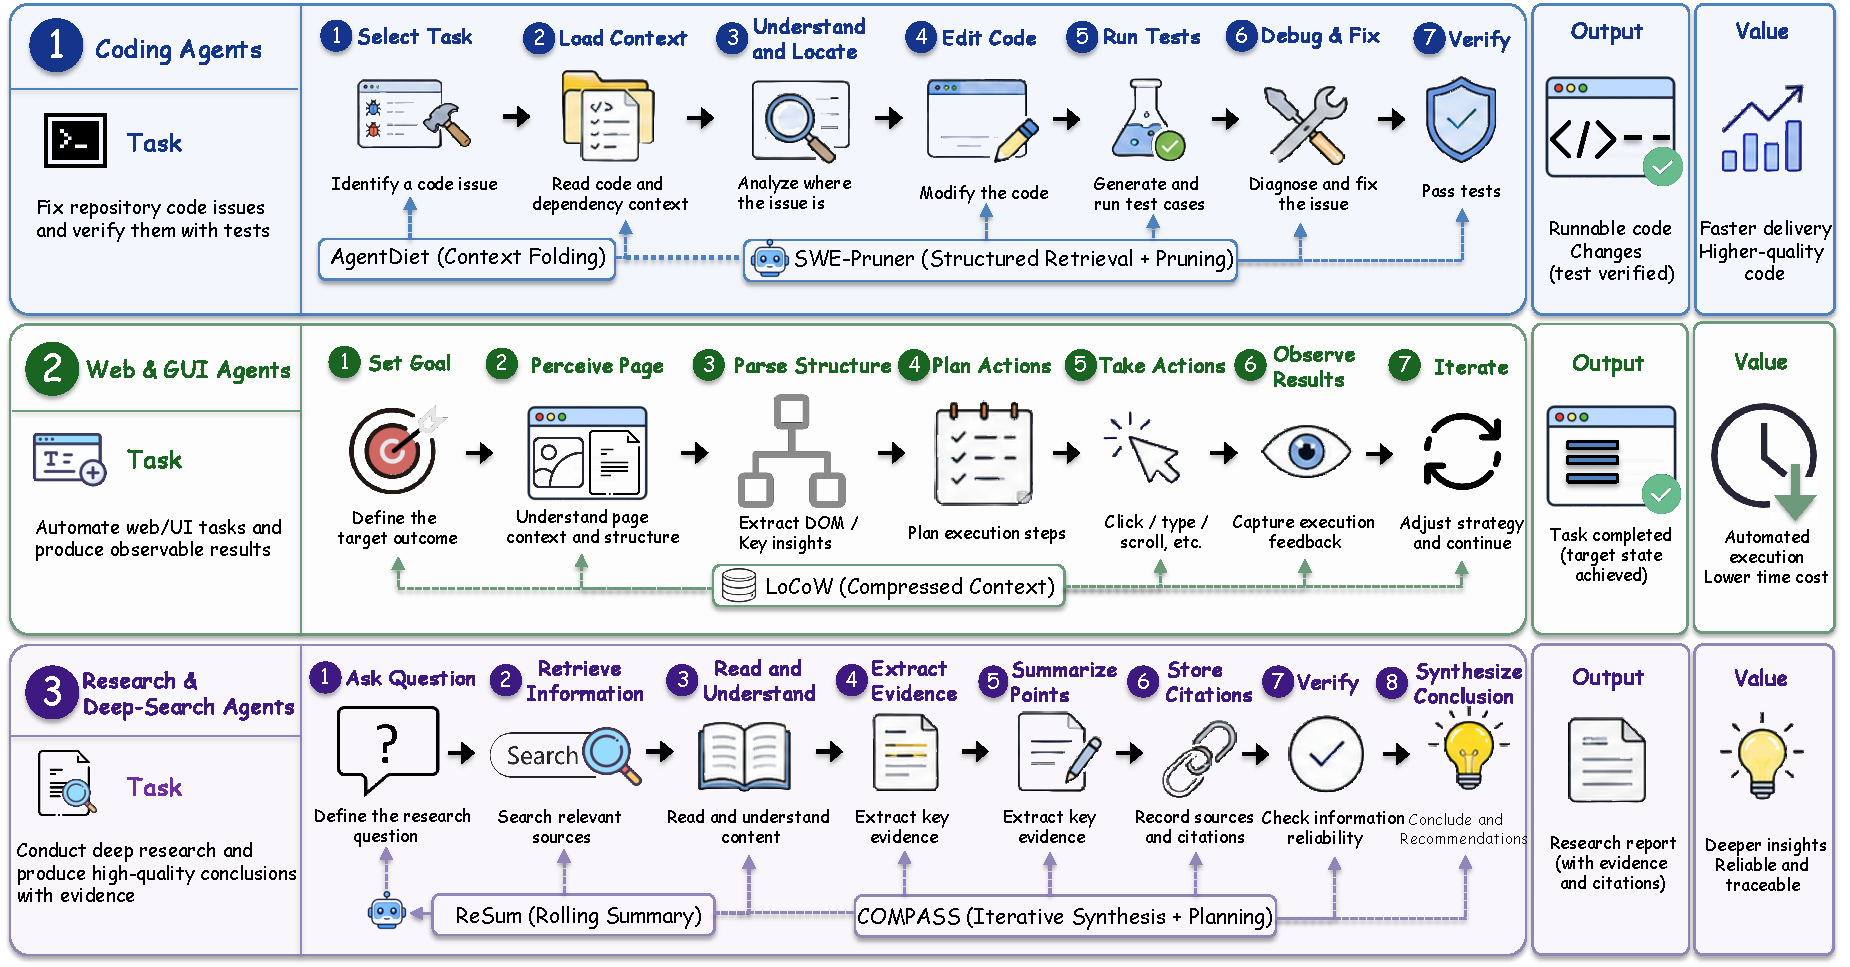
\includegraphics[width=0.8\textwidth]{figures/section6.pdf}
%      \vspace{-.2cm}
%     \caption{Domain-specific context compression regimes for coding, web/GUI, and research agents. The figure contrasts each domain's setup, workflow, interaction loop, dominant risks, and contextualized strategy choices.}
%     \label{fig:domain_specific_regimes}
% \end{figure*}

% \begin{table*}[ht]
% \centering
% \footnotesize
% \setlength{\tabcolsep}{4pt}
% \setlength{\aboverulesep}{0.2ex}
% \setlength{\belowrulesep}{0.2ex}
% \renewcommand{\arraystretch}{0.98}
% \begin{tabularx}{\textwidth}{@{}>{\raggedright\arraybackslash}p{2.2cm} >{\raggedright\arraybackslash}X >{\raggedright\arraybackslash}X >{\raggedright\arraybackslash}X >{\raggedright\arraybackslash}X@{}}
% \toprule
% \textbf{System} & \textbf{Select ($S$)} & \textbf{Compress ($\Phi$)} & \textbf{Store ($M$)} & \textbf{Recover ($R$)} \\
% \midrule
% \textbf{Claude Code} & Reactive, threshold-based selection. & Auto-compaction of prior interaction history. & Compacted state retained in active context. & Implicit recovery via continued execution. \\
% \midrule
% \textbf{Cursor} & Retrieval-first selection of files, code blocks, and rules. & Relevance filtering and contextual assembly. & Repository index, project rules, and workspace context. & Re-injection of retrieved files, rules, and evidence. \\
% \midrule
% \textbf{OpenAI Codex} & Task-grounded selection over files, instructions, and threads. & Session continuation and workspace grounding. & Task threads, instruction files, and repository state. & Recovery through continued threads and file re-access. \\
% \bottomrule
% \end{tabularx}
% \caption{Pipeline-level comparison of recent production-grade coding agents, organized by the stages in Section~\ref{subsec:unified_pipeline}.}
% \label{tab:coding_agents_pipeline}
% \end{table*}

% \noindent\textbf{\fone} refers to failures that arise before compression itself, when the system chooses the wrong moment, target, or granularity of compression. The issue is not the compression operator, but a pre-compression decision that already departs from task requirements. Typical cases include premature compression~\citep{yang2026staticsummarizationproactivememory, liu2025contexttoolcontextmanagement}, misjudging the retention value of critical information~\citep{liang2026learningremembermetacognitivemanagement, feng2026agentocrreimaginingagenthistory}, or compressing constraints that should remain exact~\citep{liu2025contexttoolcontextmanagement}. Appendix~\ref{app:case-studies-compression-failures} illustrates this pattern with a case where a compression controller prematurely removes authentication-related state before the agent reaches the step where it is required.

% \noindent\textbf{\ftwo} refers to failures introduced by the compression operation itself, where representation transformation corrupts semantics, structure, relations, constraints, or fine-grained detail. The central question is whether compression preserves the original information faithfully enough for later use. Typical cases include omitted semantics~\citep{chen2026halumemevaluatinghallucinationsmemory, yang2026staticsummarizationproactivememory}, disrupted relational structure~\citep{wu2026contextweaverselectivedependencystructuredmemory}, oversimplified constraints~\citep{chen2026halumemevaluatinghallucinationsmemory, liu2025contexttoolcontextmanagement}, or compressed uncertainty that becomes an unwarranted conclusion~\citep{yang2026staticsummarizationproactivememory}. Appendix~\ref{app:case-studies-compression-failures} provides a trajectory-level example in which compression preserves the broad task intent but loses a fine-grained constraint, causing the later agent state to become semantically incomplete.

% \noindent\textbf{\fthree} refers to failures of post-compression accessibility: information is retained in some form, but cannot be correctly retrieved, expanded, or reconstructed when needed. The issue is therefore recoverability rather than pre-compression choice or in-compression corruption. Typical cases include failed retrieval~\citep{li2026ocrmemoryopticalcontextretrieval, zeng2026kvcachecentric, chen2026halumemevaluatinghallucinationsmemory}, incorrect reconstruction~\citep{chen2026halumemevaluatinghallucinationsmemory}, or compressed states that remain storable yet functionally unusable~\citep{li2026ocrmemoryopticalcontextretrieval, zeng2026kvcachecentric}. Appendix~\ref{app:case-studies-compression-failures} shows the corresponding access-side failure: the correct compressed memory exists, but later retrieval returns a semantically similar yet wrong memory item.

% Together, \textbf{F1}–\textbf{F3} define a temporal failure taxonomy over the compression pipeline. For hybrid cases, we assign the label to the earliest failure that causally triggers later errors, since agent workflows naturally exhibit error propagation~\citep{wang2024survey}.


% % We synthesized the existing literature on context compression failure modes and organized them into an exhaustive and non-overlapping taxonomy along the temporal sequence of compression, which are {\fone}, {\ftwo} and {\fthree}, respectively, as illustrated in Figure~\ref{fig:failure_modes_taxonomy}.

% % \begin{figure*}[t]
% %     \centering
% %     
\includegraphics[width=0.85\textwidth]{figures/section5.pdf}
% %     \caption{A temporal taxonomy of context compression failures. Failures are classified by the earliest point at which they occur in the compression pipeline: {\fone}, {\ftwo}, and {\fthree}.}
% %     \label{fig:failure_modes_taxonomy}
% % \end{figure*}

% % \paragraph{\fone} refers to failures arising before compression is performed, where the system makes incorrect decisions regarding whether to compress, when to compress, what information should be compressed, and at what granularity compression should occur. The core issue in this category does not lie in the correctness of the compression operation itself, but rather in the fact that the upstream decision-making process has already deviated from task requirements. Typical examples include compressing information prematurely~\citep{yang2026staticsummarizationproactivememory, liu2025contexttoolcontextmanagement}, misjudging the retention value of critical information~\citep{liang2026learningremembermetacognitivemanagement, feng2026agentocrreimaginingagenthistory}, or incorporating core constraints that should remain intact into the compression process~\citep{liu2025contexttoolcontextmanagement}, thereby leading to subsequent information loss or contextual mismatch during execution.

% % \paragraph{\ftwo} refers to failures in which the compression operation itself causes information corruption during the process of representation transformation, resulting in substantial loss of the original content’s semantics, structure, relationships, constraints, or fine-grained details in the compressed representation. The core issue in this category does not concern whether the pre-compression decision was appropriate, but rather whether the compression process faithfully preserves the original information. Typical examples include the omission of critical semantics~\citep{chen2026halumemevaluatinghallucinationsmemory, yang2026staticsummarizationproactivememory}, the disruption of relational structures~\citep{wu2026contextweaverselectivedependencystructuredmemory}, the over-simplification of constraint conditions~\citep{chen2026halumemevaluatinghallucinationsmemory, liu2025contexttoolcontextmanagement}, or the erroneous compression of uncertainty in the original content into overly definitive conclusions~\citep{yang2026staticsummarizationproactivememory}, thereby preventing the compressed representation from fully supporting subsequent reasoning and execution.

% % \paragraph{\fthree} refers to failures in which compressed information has technically been retained in some form, yet cannot be correctly retrieved, accessed, expanded, or reconstructed during subsequent use. The core issue in this category lies neither in whether the pre-compression decision was appropriate nor in whether the compression process itself introduced information corruption, but rather in failures of post-compression accessibility and recoverability. Typical examples include situations where information still exists but cannot be successfully retrieved~\citep{li2026ocrmemoryopticalcontextretrieval, zeng2026kvcachecentric, chen2026halumemevaluatinghallucinationsmemory}, where retrieved information is reconstructed incorrectly~\citep{chen2026halumemevaluatinghallucinationsmemory}, or where the compressed representation remains formally storable yet functionally unusable~\citep{li2026ocrmemoryopticalcontextretrieval, zeng2026kvcachecentric}, thereby preventing the originally preserved content from being effectively utilized in downstream tasks.

% % In summary, \ensuremath{F^{1}}–\ensuremath{F^{3}} collectively constitute a complete causal chain of context compression failures in temporal order. The three categories are naturally distinguished by their positions within the failure pipeline. By classifying each failure according to the earliest and most critical point at which the error occurs, the framework can maintain both mutual exclusivity and overall completeness. For hybrid cases involving multiple issues simultaneously, priority should be given to annotating the earliest failure source that causally triggers subsequent errors, since agent workflows inherently exhibit error propagation characteristics~\citep{wang2024survey}.